\documentclass[a4paper]{article}

\usepackage{fullpage} % Package to use full page
\usepackage{parskip} % Package to tweak paragraph skipping
\usepackage{tikz} % Package for drawing
\usepackage{amsmath}
\usepackage{hyperref}
\usepackage{ctex}
\usepackage{listings}

%导言区的此三行无变化
\usepackage{graphicx}
\usepackage{float} 
\usepackage{subfigure}
\usepackage{caption}
\usepackage{tabularx}

\renewcommand\thefigure{\thesection.\arabic{figure}}
\makeatletter
\@addtoreset{figure}{section}
\makeatother

\renewcommand\thetable{\thesection.\arabic{table}}
\makeatletter
\@addtoreset{table}{section}
\makeatother

\makeatletter
\renewcommand \theequation {%
	\ifnum \c@section>\z@ \@arabic\c@section.\fi \ifnum \c@subsection>\z@
	\@arabic\c@subsection.\fi\ifnum \c@subsubsection>\z@
	\@arabic\c@subsubsection.\fi\@arabic\c@equation}
\@addtoreset{equation}{section}
\@addtoreset{equation}{subsection}
%\setcounter{section}{-1}
\makeatother
\captionsetup[figure]{labelfont={bf},name={Fig.},labelsep=period}
\captionsetup[table]{labelfont={bf},name={Table.},labelsep=period}
\setlength{\parindent}{2em}

\lstset{
	columns=fixed,       
	numbers=left,                                        % 在左侧显示行号
	numberstyle=\tiny\color{gray},                       % 设定行号格式
	frame=none,                                          % 不显示背景边框
	backgroundcolor=\color[RGB]{245,245,244},            % 设定背景颜色
	keywordstyle=\color[RGB]{40,40,255},                 % 设定关键字颜色
	numberstyle=\footnotesize\color{darkgray},           
	commentstyle=\it\color[RGB]{0,96,96},                % 设置代码注释的格式
	stringstyle=\rmfamily\slshape\color[RGB]{128,0,0},   % 设置字符串格式
	showstringspaces=false,                              % 不显示字符串中的空格
	language=c++,                                        % 设置语言
}


\begin{document}

%\maketitle
\newcommand{\HRule}{\rule{\linewidth}{0.5mm}}
\begin{titlepage}
	\begin{center}
		% Upper part of the page
		
\includegraphics[width=0.4\textwidth]{Tsinghua2.png}\\[1cm]
		\textsc{\Large \texttt{清华大学电子工程系}}\\[1cm]
		% Title
		\HRule \\[1cm]
		{\Huge \bfseries 大数据分析B作业1}\\[0.4cm]
		\HRule \\[3.5cm]
		% Author and supervisor
		\begin{minipage}{0.4\textwidth}
			\begin{center}
				\Large
				\begin{tabular}{cc}
					\texttt{作者:} & 罗雁天 \\[0.5cm]
					\texttt{学号:} & 2018310742 \\[0.5cm]
					\texttt{日期:} & \today
				\end{tabular}
			\end{center}
		\end{minipage}
		\vfill
	\end{center}
\end{titlepage}


%\tableofcontents
\newpage

\section{Recall and Write down the assumption which one-way ANOVA are based on.}


\textbf{ANSWER}

\begin{itemize}
	\item The data are randomly sampled;
	\item The variance of each group are assumed equal;
	\item The residual are normly distributed;
\end{itemize}

\section{Focus on two columns: Category (Col[2]) and Average Age (Col[7]). Taking feature Average Age as an example, we want to measure whether the average age varied significantly across the categories. Clearly state the null (H0) and the alternative (H1) hypotheses for this task.}


\textbf{ANSWER}

The null($H_0$) and the alternative ($H_1$) are:
\begin{itemize}
	\item $H_0$: there is no interaction between the average age and the categories;
	\item $H_1$: the average age varies significantly across the categories.
\end{itemize}

\section{Use your favorite statistics analysis software, like Matlab, R, Excel, SPSS or ...}


\subsection{Draw the empirical probability density function of Col[7], i.e. the empirical pdf of average age. Does the data in this dimension follow Gaussian distribution? Test normality of Col[7]}
\label{subsec:3a}
\textbf{ANSWER}

The empirical pdf of Col[7] is in Fig.\ref{3a} 
\begin{figure}[h]
	\centering
	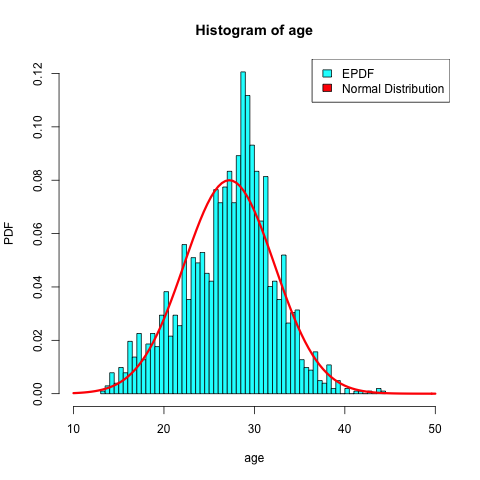
\includegraphics[width=0.7\linewidth]{images/3a.png}
	\caption{\label{3a}Empirical pdf of Col[7] data}
\end{figure}

We also draw the Gaussian distribution in Fig.\ref{3a} for comparison. Intuitively, we can find that the data in Col[7] does not follow Gaussian distribution.

\textbf{Normality test:}

We use Anderson-Darling normality test to test the normality. More detailed, we use function \textbf{ad.test()} in \textbf{nortest} package in \textbf{R} to test the normality.  The assumption is:
\begin{itemize}
	\item $H_0$: the data are normly distributed.
	\item $H_1$: the data are not normly distributed.
\end{itemize}

The result of the test is in Fig.\ref{3a2}, we can see $A=9.3826, p-value<2.2e-16$, therefore, the data in Col[7] does not follow Gaussian distribution.
\begin{figure}[h]
	\centering
	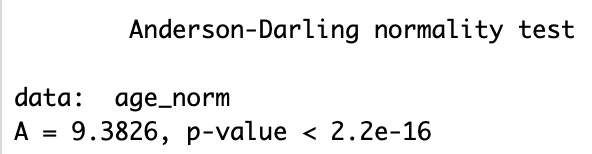
\includegraphics[width=0.7\linewidth]{images/3a2.png}
	\caption{\label{3a2}The result of normality test}
\end{figure}

The code for this question is in "code/3a.R"

\subsection{In Col[7], there are 5 components divided by category labels. We denote the data in Col[7] with category i (where i = 1,...,5) as Col[7| categoty=i]. Test the normality of each components and test the homogeneity of variances.}

\textbf{ANSWER}

Using the Anderson-Darling normality test like section \ref{subsec:3a}, we can get the results(at 5\% level) in Table \ref{tab:table1}

\begin{table}[htbp]
	\centering
	\caption{The results of normality test for each catebory}
	\label{tab:table1}
	\begin{tabular}{|c|c|c|c|c|c|}
		\hline
		Category & 1 & 2 & 3 & 4 & 5 \\
		\hline
		p-value & 0.02513 & 0.003444 & 0.2225 & 1.088e-05 & 2.2e-16 \\
		\hline
		Normality & No & No & Yes & No & No \\
		\hline
	\end{tabular}
\end{table}

To test the homogeneity of variances, our assumption is:
\begin{itemize}
	\item $H_0$: The variances of each group are equal
	\item $H_1$: The variances of each group are not equal.
\end{itemize}

We use Bartlett test of homogeneity of variances, the result is in Fig.\ref{3b1}, we can see $p\_value < 2.2\times10^{-16}$, therefore we reject the null assumption, i.e., the variances of each group is not equal.

\begin{figure}[h]
	\centering
	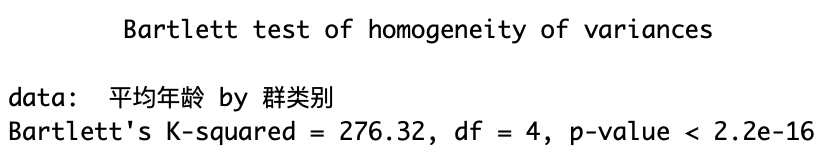
\includegraphics[width=0.7\linewidth]{images/3b.png}
	\caption{\label{3b1}The result of the test of homogeneity of variances}
\end{figure}

The code for this question is in "code/3b.R"

\subsection{Do the one-way ANOVA test for Col[7] with categories in Col[2]. Write down your conclusion, supporting statistics, and visualize your data which inspire the process.}
\label{subsec:3c}
\textbf{ANSWER}



Using the function \textbf{anova1} in \textbf{MATLAB}, we can get the result of the one-way ANOVA test as Fig.\ref{3c}
\begin{figure}[h]
	\centering
	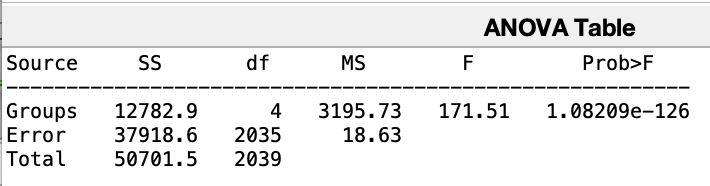
\includegraphics[width=0.8\linewidth]{images/3c.png}
	\caption{\label{3c}The result of the ANOVA test}
\end{figure}

With significance level of 5\%, because $p\_value=1.08209\times 10^{-126}<0.05$, wo reject the null assumption. Thus the average age varies significantly across the categories.

We also draw the box plot of each group as Fig.\ref{3c2}. Intuitively, we can find that the center lines of the
boxes have large differences, which indicate the average age varies significantly across the categories.

\begin{figure}[h]
	\centering
	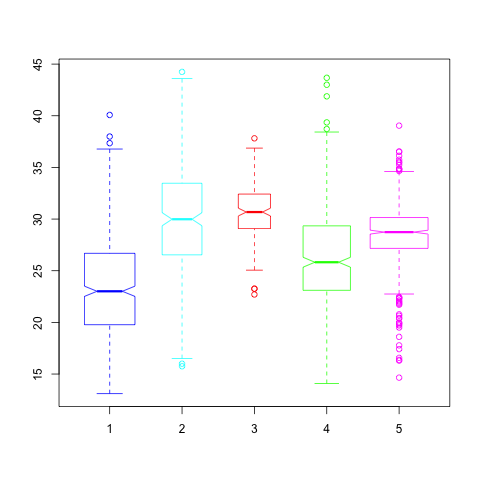
\includegraphics[width=0.9\linewidth]{images/3c3.png}
	\caption{\label{3c2}The box plot of each group}
\end{figure}

The code for this question is in "code/3c.R" and "code/problem3c.m"

\section{Choose another 3 columns, draw the empirical pdf of each feature columns and test which column follows these assumptions in question 1? How about their corresponding log transformation?}

\textbf{ANSWER}
We choose Col[6](性别比), Col[13](夜聊比例), Col[14](图片比例) data in this question. The empirical pdf of each feature columns as in Fig.\ref{41} and the empirical pdf of their log transformation as in Fig.\ref{42}. In Fig.\ref{42}, we do not show the epdf of their log transformation if the data=0.

\begin{figure}[h]
	\centering
	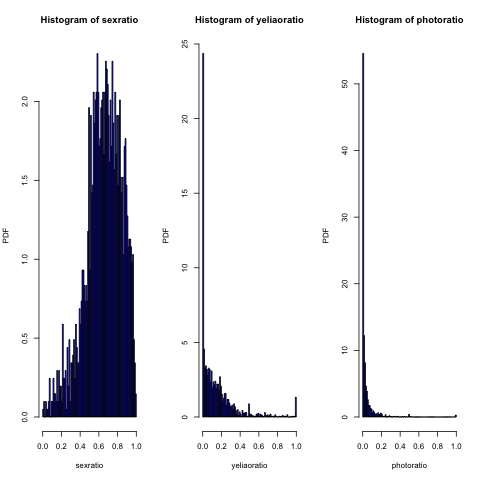
\includegraphics[width=0.9\linewidth]{images/41.png}
	\caption{\label{41}The Empirical pdf of Col[6], Col[13] and Col[14]}
\end{figure}

\begin{figure}[h]
	\centering
	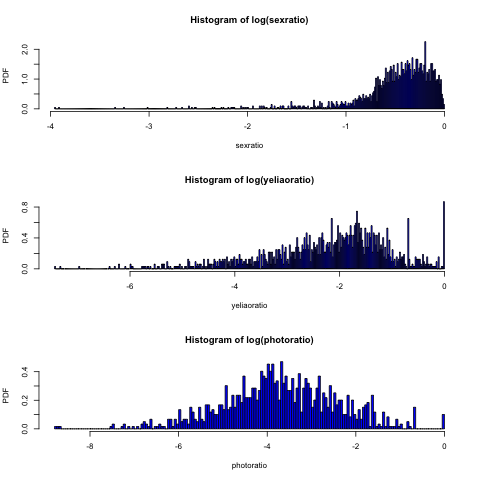
\includegraphics[width=0.9\linewidth]{images/42.png}
	\caption{\label{42}The Empirical pdf of log transformation of Col[6], Col[13] and Col[14]}
\end{figure}

Then we test normality (Anderson-Darling normality test) and the homogeneity of variances (Barlett Test) of the data in Col[6], Col[13], Col[14] and their log transformation. With significance level of 5\%, the result is in Table\ref{tab:table2}

\begin{table}[htbp]
	\centering
	\caption{The results of normality test and homogeneity of variances test for Col[6,13,14]}
	\label{tab:table2}
	\begin{tabular}{|c|c|c|c|c|c|c|}
		\hline
		Results & Col[6] & Col[13] & Col[14] & log(Col[6]) & log(Col[13]) & log(Col[14]) \\
		\hline
		Normality p-value & 2.2e-16 & 2.2e-16 & 2.2e-16 & 2.2e-16 & 2.2e-16 & 2.2e-16\\
		\hline
		Normality & No & No & No & No & No & No\\
		\hline
		Homogeneity p-value & 2.2e-16 & 2.2e-16 & 2.2e-16 & 2.2e-16 & 0.0003192 & 0.504 \\
		\hline
		Homogeneity & No & No & No & No & No & Yes \\
		\hline
	\end{tabular}
\end{table}

The code for this question is in "code/4.R"

\section{How to do one-way ANOVA with the non-normal data?}
\subsection{Find and list the possible solutions set.}
\textbf{ANSWER}

\begin{itemize}
	\item We can use some algorithms to transform non-normal data into the Gaussian distributed shape.
	\item We can use the non-parametric Kurskal-Wallis Test, which does not require the normality assumption.
	\item Last but not least, the one-way ANOVA can tolerate non-normal data (skewed or kurtotic) with a small effect on the Type1 error rate, thus we can use Type1 error rate to do the one-way ANOVA.
\end{itemize}

\subsection{Do the one-way ANOVA on the 3 columns you choose. Do these
	feature columns vary significantly? Visualize the results.}
\textbf{ANSWER}

Like the method in section\ref{subsec:3c}, we can get the results as followed:

For the data in col[6], the result is in Fig.\ref{5b01} and Fig.\ref{5b1}.With significance level of 5\%, because $p\_value=2.53208\times 10^{-43}<0.05$, wo reject the null assumption. Thus the average age varies significantly across the categories. And from the box plot, we can find that the center lines of the
boxes have large differences, which indicate the average age varies significantly across the categories.


For the data in col[13], the result is in Fig.\ref{5b02} and Fig.\ref{5b2}.With significance level of 5\%, because $p\_value=9.893\times 10^{-23}<0.05$, wo reject the null assumption. Thus the average age varies significantly across the categories. And from the box plot, we can find that the center lines of the
boxes have large differences, which indicate the average age varies significantly across the categories.

For the data in col[14], the result is in Fig.\ref{5b03} and Fig.\ref{5b3}.With significance level of 5\%, because $p\_value=0.006<0.05$, wo reject the null assumption. Thus the average age varies significantly across the categories. And from the box plot, we can find that the center lines of the
boxes have large differences, which indicate the average age varies significantly across the categories.

The code for this question is in "code/5b.R" and "code/problem5b.m"

\begin{figure}[!h]
	\centering
	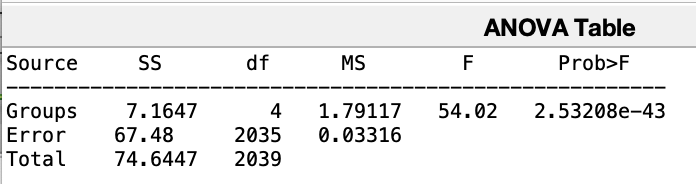
\includegraphics[width=\linewidth]{images/5b01.png}
	\caption{\label{5b01}The result of ANOVA test on Col[6]}
\end{figure}
\begin{figure}[!h]
	\centering
	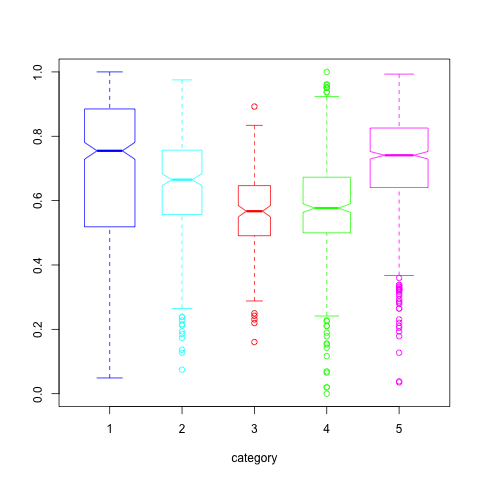
\includegraphics[width=\linewidth]{images/5b1.png}
	\caption{\label{5b1}The box plot of each group on Col[6]}
\end{figure}
\begin{figure}[!h]
	\centering
	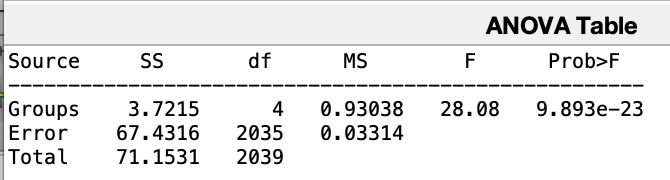
\includegraphics[width=\linewidth]{images/5b02.png}
	\caption{\label{5b02}The result of ANOVA test on Col[13]}
\end{figure}
\begin{figure}[!h]
	\centering
	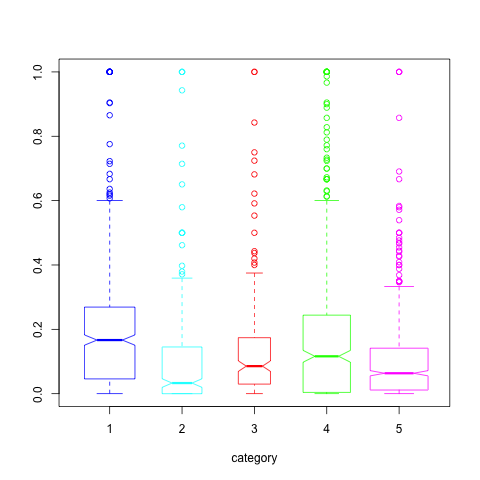
\includegraphics[width=\linewidth]{images/5b2.png}
	\caption{\label{5b2}The box plot of each group on Col[13]}
\end{figure}
\begin{figure}[!h]
	\centering
	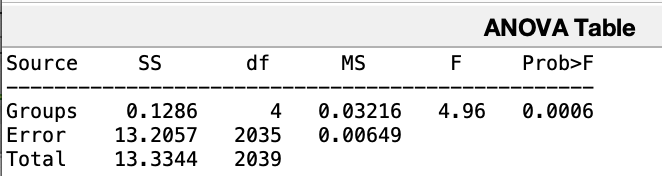
\includegraphics[width=\linewidth]{images/5b03.png}
	\caption{\label{5b03}The result of ANOVA test on Col[14]}
\end{figure}
\begin{figure}[!h]
	\centering
	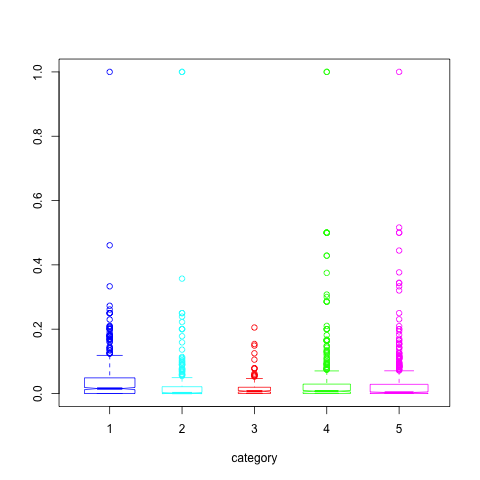
\includegraphics[width=\linewidth]{images/5b3.png}
	\caption{\label{5b3}The box plot of each group on Col[14]}
\end{figure}



\section{Redo the ANOVA test in question 3 c) by sampling 10\% data (i.e. around 200 groups). Repeat 10 times and compute the mean and standard deviation of the supporting statistics (F value). Compare at least two sampling strategies. Which sampling method is more stable? How are the results compared to the results without sampling? Why?}

\textbf{ANSWER}

Here we use Simple Random Sampling, Stratified Random Sampling and Systematic Random Sampling for comparison. The results of 10 times F\_values, means and standard deviations are shown in Table\ref{tab:table3}

\begin{table}[htbp]
	\centering
	\caption{F values, means and stds of 10 times for 3 sampling strategies}
	\label{tab:table3}
	\begin{tabular}{|c|c|c|c|c|c|c|c|c|c|c|c|c|}
		\hline
		Samplings & 1 &2 &3 &4 &5 &6 & 7 &8 & 9 &10 & mean & std \\
		\hline
		Simple & 31.78 & 17.11 & 17.37 & 34.08 & 15.97 & 12.18 & 16.42 & 15.49 & 12.65 & 29.97 & 20.30 & 8.26\\
		\hline
		Stratified & 17.29 & 22.13 & 20.39 & 12.39 & 15.83 & 15.49 & 18.48 & 17.19 & 9.69 & 23.62 & 17.25 & 4.23\\
		\hline
		Systematic & 28.44 & 11.38 & 11.38 & 11.38 & 13.58 & 16.65 & 20.65 & 25.24 & 9.58 & 25.24 & 17.35 & 6.99 \\
		\hline
	\end{tabular}
\end{table}

From Table\ref{tab:table3}, we can find that Stratified Random Sampling is more stable because it has smallist standard deviation. Compared to the results without sampling in Fig.\ref{3c}(F0=171.51), the sampling results are about 10\% of the F0. Recall the F formula:
\begin{equation}
F=\frac{MS_{Between}}{MS_{Within}}=\frac{SS_b\cdot db_w}{SS_w\cdot df_b}
\end{equation}
In the calculation of sampling, $SS_b$ and $SS_w$ calculations only consider 10\% of total data, $df_b$ is still 4 and $db_w=204-5=199$ (nearly 10\% of 2040-5). Therefore, the F-stats with sampling is nearly 10\% of the F-stats without sampling.

The code for this question is in "code/problem6.m"

\section{Choose any two categories, and classify them by logistical regression, or you can try multi-label classification on all categories.}

\textbf{ANSWER}

First we choose category 1 and category 2 for logistical regression. We assign $label=0$ if the group is in category 1 else assign $label=1$. We use cross\_entropy in equation \ref{eq1} as our loss function and we use Gradient Descent to optimize weight w in logistical regression. We set $learning rate=0.1$ and $iter_num=2000$, we get the accurcay curve and the loss curve in Fig.\ref{7}. And the last accuracy is 76.9\%.

\begin{equation}
\label{eq1}
loss = -\sum_{i=1}^{n}(y_i\log p_i +(1-y_i)\log(1-p_i))
\end{equation}

\begin{figure}[!h]
	\centering
	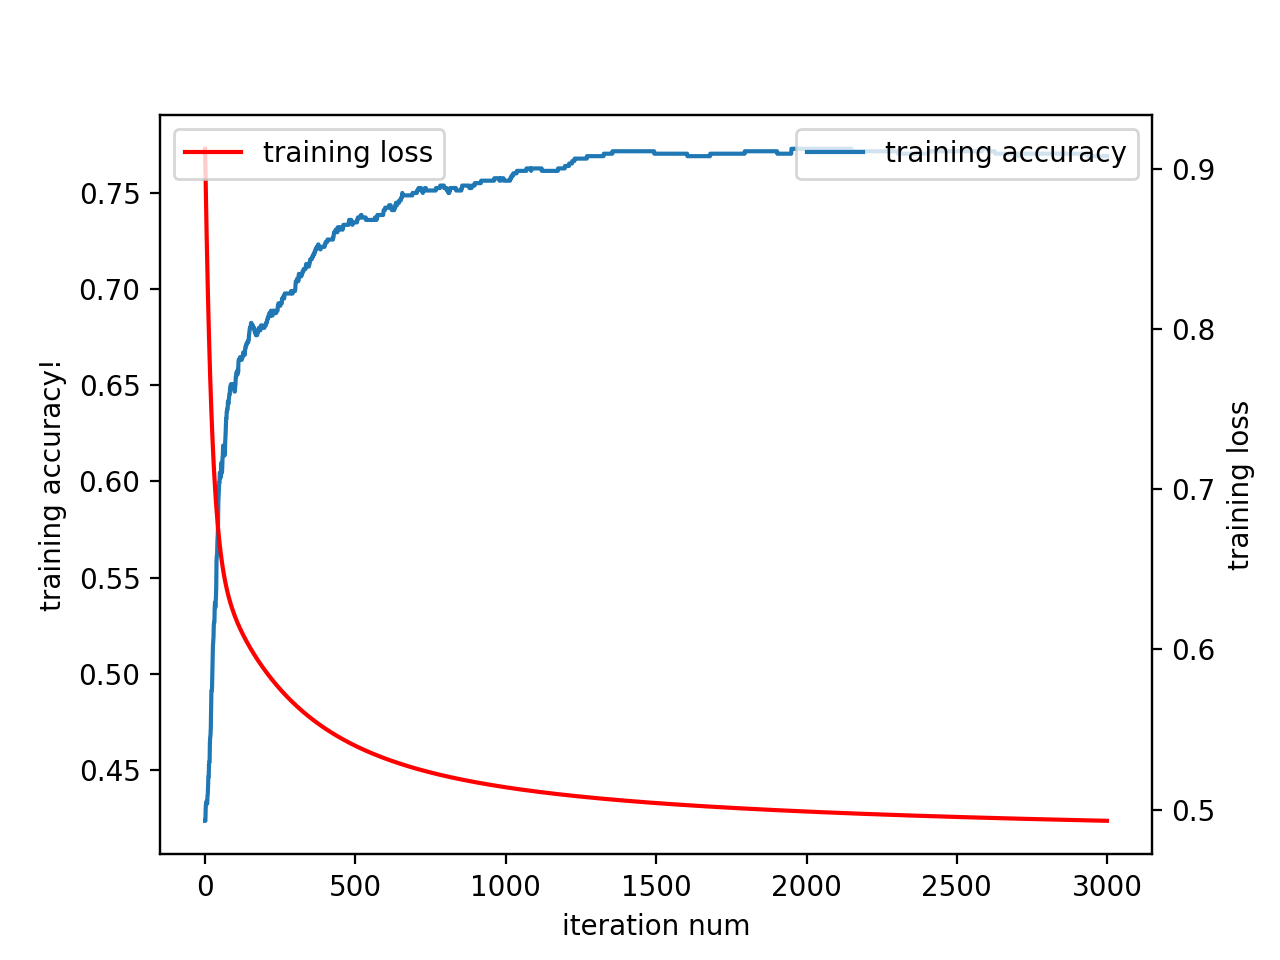
\includegraphics[width=\linewidth]{images/7.png}
	\caption{\label{7}The training accuracy and training loss of logistical regression on category 1 and coregory 2}
\end{figure}

Then we only take the Col[7](平均年龄), Col[8](年龄差) of category 1, 2 and we classify them by logistical regression and we draw the classification border of the two categories as shown in Fig.\ref{73}. And the last accuracy is 75.8\%, the accurcay curve and the loss curve in Fig.\ref{72}. From the result, 75.8\% is nearly 76.9\%, we can find the two categories mostly differ in age.

\begin{figure}[h]
	\centering
	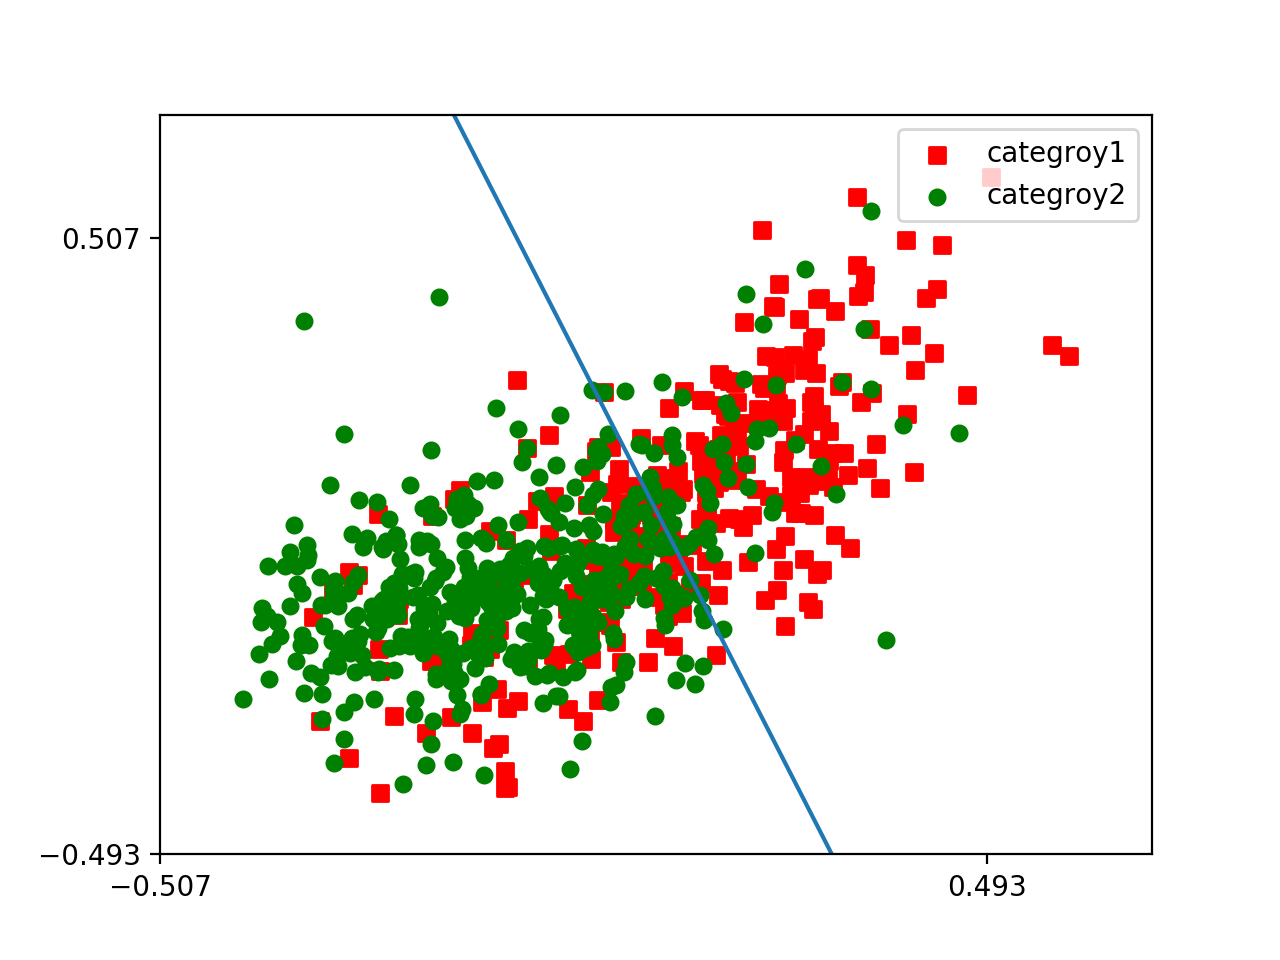
\includegraphics[width=0.8\linewidth]{images/73.png}
	\caption{\label{73}The classification border of category 1,2 on Col[7], Col[8]}
\end{figure}

\begin{figure}[h]
	\centering
	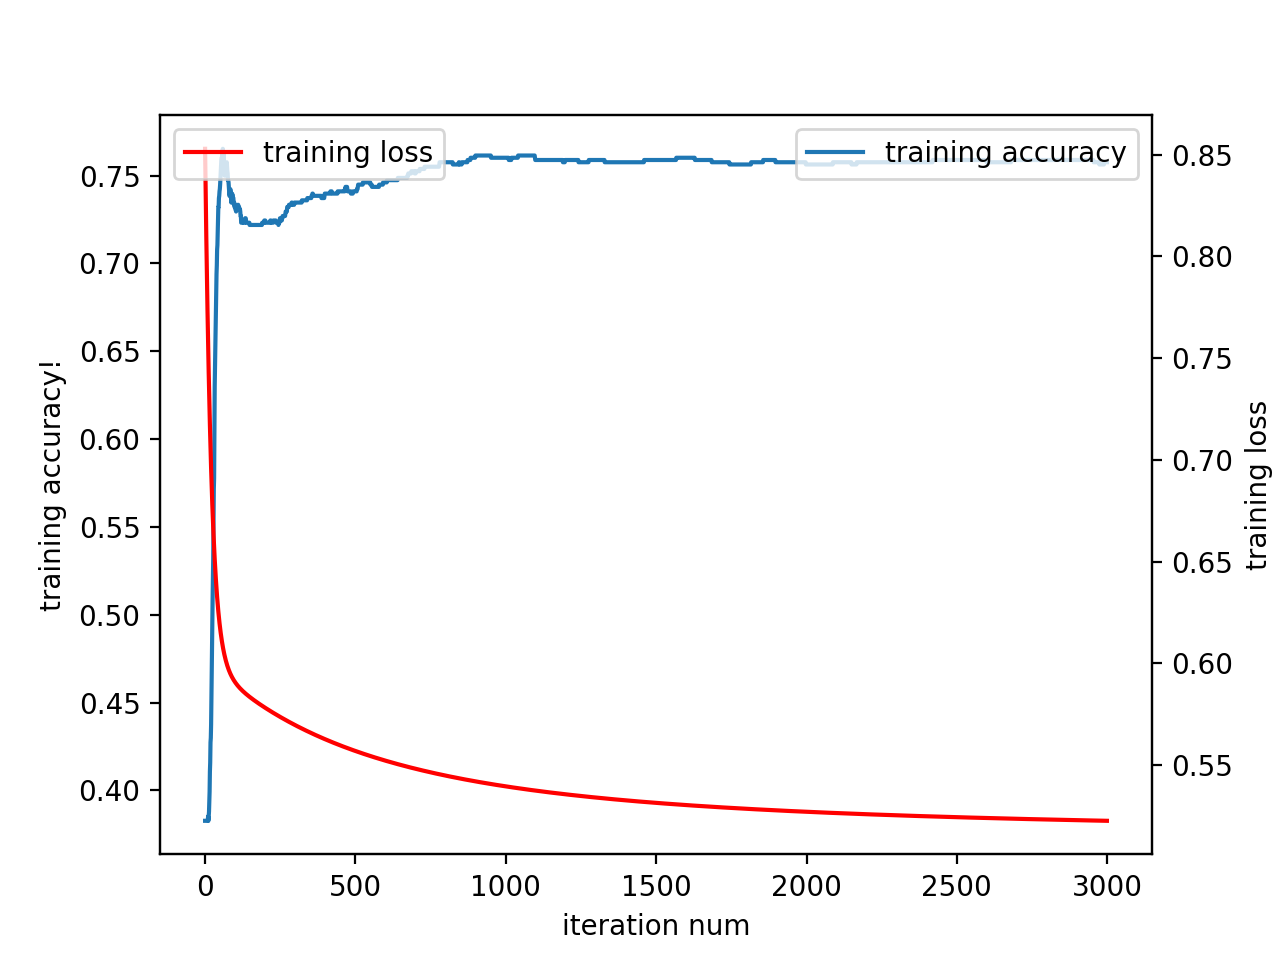
\includegraphics[width=0.8\linewidth]{images/72.png}
	\caption{\label{72}The training accuracy and training loss of logistical regression on category 1 and coregory 2 with only Col[7], Col[8]}
\end{figure}

The code for this question is in "code/problem7.py"

\end{document}